\newpage
\section{Introduction}
\label{sec:introduction}
% state the learning objective 

The objective of this laboratory assignment is to study a circuit containing dependent and independent sources of both voltage and current alonside various resistors (2 dependent sources, 2 independent souces and 7 resistors to be more precise). To do so we've obtained the current in the various meshes and the voltage in all the nodes, using two diferent methods alongside a simlulation to corroborate the results.


The circuit that will be analysed is represented in the image below and the values of each constant are especifed in the table below.

\begin{figure}[ht]
\centering
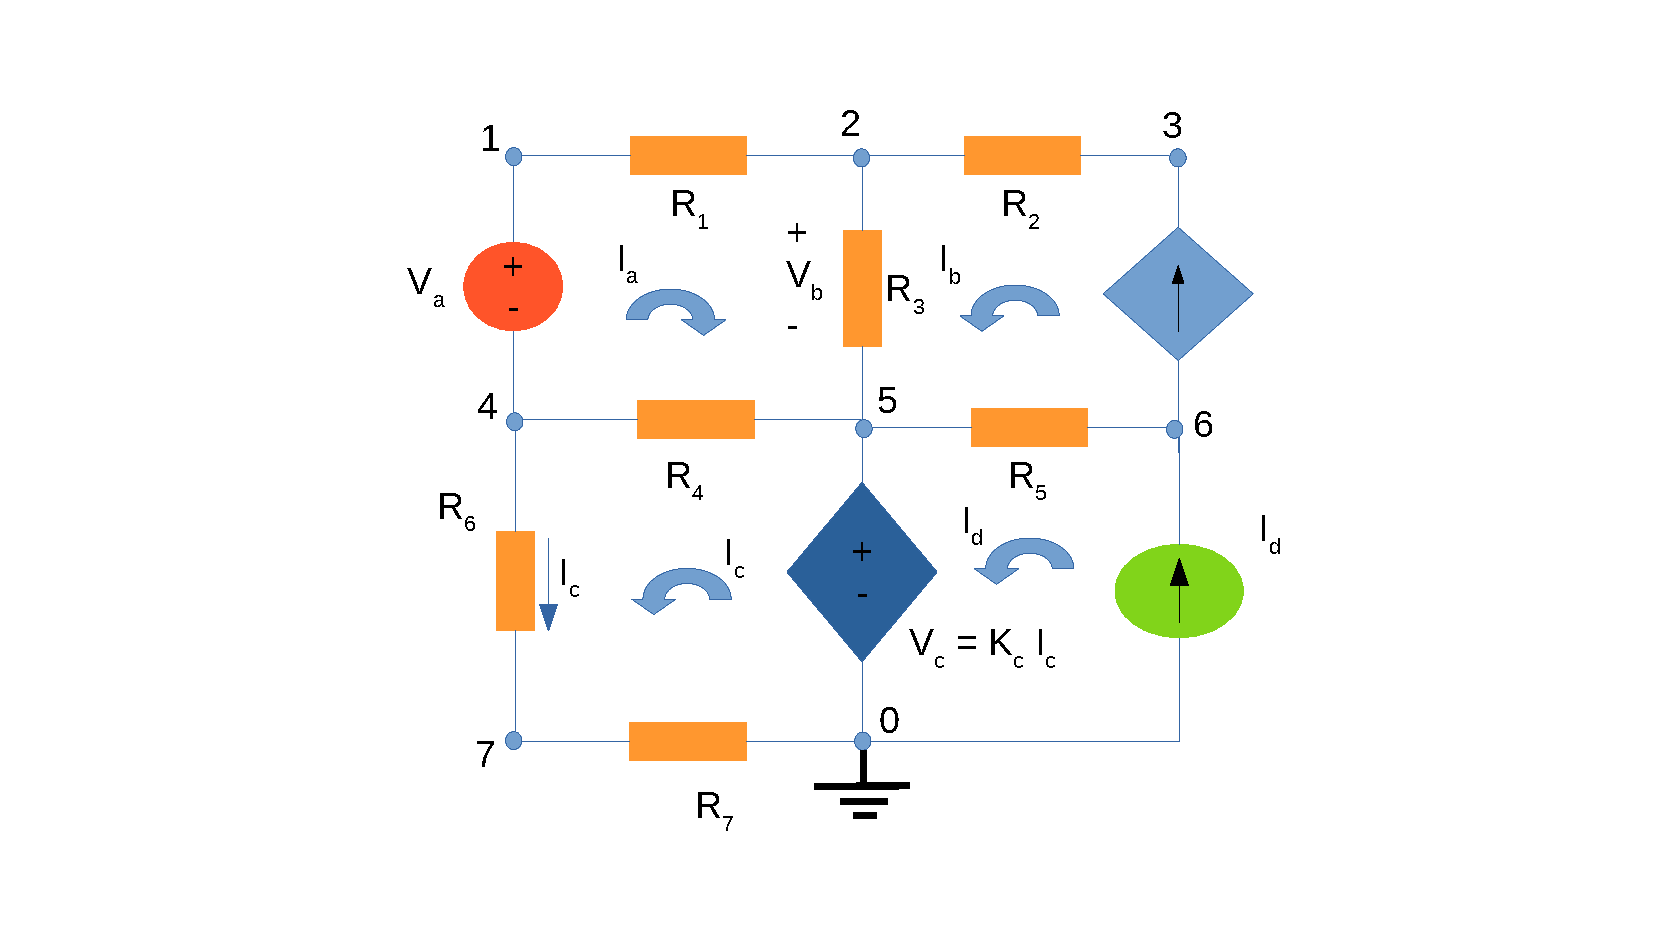
\includegraphics[width = 15cm]{system2.pdf}
\caption {Circuit}
\end{figure}


\begin{table}[ht] \centering
\begin{tabular}{|
>{\columncolor[HTML]{FFCC67}}l |c|}
\hline
{\color[HTML]{333333} R1}               & 1.013609e+00 kOhm            \\ \hline
{\color[HTML]{333333} R2}               & 2.016578e+00 kOhm             \\ \hline
{\color[HTML]{333333} R3}               & 3.006816e+00 kOhm             \\ \hline
{\color[HTML]{333333} R4}               & 4.049229e+00 kOhm            \\ \hline
{\color[HTML]{333333} R5}               & 3.053925e+00 kOhm             \\ \hline
{\color[HTML]{333333} R6}               & 2.092502e+00 kOhm             \\ \hline
{\color[HTML]{333333} R7}               & 1.022320e+00 kOhm             \\ \hline
{\color[HTML]{333333} Id}               & 1.029587e+00 mA               \\ \hline
{\color[HTML]{333333} Kb}               & 7.213324e+00 mA/V             \\ \hline
{\color[HTML]{333333} Kc}               & 8.321035e+00 mA/V             \\ \hline
\end{tabular}
\caption{Initial info}
\end{table}


In Section~\ref{sec:analysis}, a theoretical analysis of the circuit is
presented. In Section~\ref{sec:simulation}, the circuit is analysed by
simulation, and the results are compared to the theoretical results obtained in
Section~\ref{sec:analysis}. The conclusions of this study are outlined in
Section~\ref{sec:conclusion}. \\

\pagebreak
